\documentclass[../PianoDiProgetto.tex]{subfiles}
\begin{document}
	\section{Preventivo}
		\subsection{Analisi}
			\subsubsection{Prospetto orario}
			\begin{table}[H]
			\center
				\begin{tabular}{cccccccc}
				\noalign{\hrule height 1.5pt}
				\textbf{Nome} & \textbf{Res} & \textbf{Amm} & \textbf{An} & \textbf{Pt} & \textbf{Pr} & \textbf{Ve} & \textbf{Totale} \\ \hline
				Bonato Enrico & - & 5 & 10 & - & - & 3 & 18 \\ \hline
				Bonolo Marco  & - & - & 8 & - & - & 7 & 15 \\ \hline
				Pace Giulio  & - & 5 & 8 & - & - & 5 & 18 \\ \hline
				Pezzuto Francesco  & - & - & 9 & - & - & 8 & 17 \\ \hline
				Sanna Giovanni  & 7 & - & 9 & - & - & 4 & 20 \\ \hline
				Sovilla Matteo  & 7 & - & 5 & - & - & 5 & 17  \\ \hline
				\textbf{Ore Totali Ruolo} & \textbf{14} & \textbf{10} & \textbf{49} & \textbf{0} & \textbf{0} & \textbf{32} & \textbf{105} \\ \hline
				\noalign{\hrule height 1.5pt}
				\end{tabular}
			\caption{Prospetto orario Analisi.  \label{tab:table_label}}
			\end{table}
			\begin{figure}[H]
				\centering
				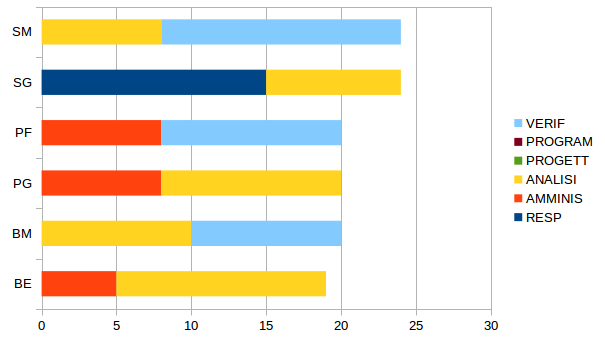
\includegraphics[scale=0.7]{Figures/OreComponenteAnalisi.png}
				\caption{Analisi: ore per componente.}\label{fig:1}
			\end{figure}
			\begin{figure}[H]
				\centering
				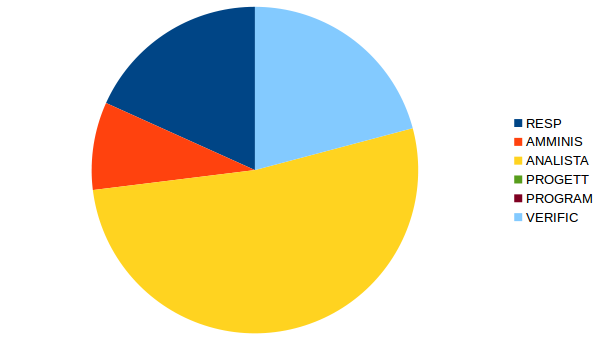
\includegraphics[scale=0.7]{Figures/OreRuoloAnalisi.png}
				\caption{Analisi: ore per ruolo.}\label{fig:2}
			\end{figure}
			
			\subsubsection{Prospetto economico}
			\begin{table}[H]
				\center
				\begin{tabular}{|c|c|c|}
					\noalign{\hrule height 1.5pt}
					\textbf{Ruolo} & \textbf{Ore} & \textbf{Costo(\euro)}     \\
					\hline
					Responsabile  & 14 & 420\\ 
					\hline
					Amministratore  & 10  & 200\\
					\hline
					Analista  & 49 & 1225\\
					\hline
					Progettista  & 0 & 0\\
					\hline
					Programmatore  & 0 & 0\\
					\hline
					Verificatore  & 32 & 480\\
					\hline
					\textbf{Totale}  & \textbf{105} & \textbf{2325}\\
					\noalign{\hrule height 1.5pt}
			\end{tabular}
			\caption{Prospetto economico Analisi.  \label{tab:table_label}}
		\end{table}
		
		\subsection{Analisi di dettaglio}
			\subsubsection{Prospetto orario} 
			\begin{table}[H]
			\center
				\begin{tabular}{cccccccc}
				\noalign{\hrule height 1.5pt}
				\textbf{Nome} & \textbf{Res} & \textbf{Amm} & \textbf{An} & \textbf{Pt} & \textbf{Pr} & \textbf{Ve} & \textbf{Totale} \\ \hline
				Bonato Enrico & 5 & - & - & - & - & - & 5 \\ \hline
				Bonolo Marco  & - & - & - & - & - & 6 & 6 \\ \hline
				Pace Giulio  & - & - & - & - & - & 6 & 6 \\ \hline
				Pezzuto Francesco  & - & - & 6 & - & - & - & 6 \\ \hline
				Sanna Giovanni  & - & - & 5 & - & - & - & 5 \\ \hline
				Sovilla Matteo  & - & 5 & - & - & - & - & 5 \\ \hline
				\textbf{Ore Totali Ruolo} & \textbf{5} & \textbf{5} & \textbf{11} & \textbf{0} & \textbf{0} & \textbf{12} & \textbf{33} \\ \hline
				\noalign{\hrule height 1.5pt}
				\end{tabular}
			\caption{Prospetto orario Analisi di dettaglio.  \label{tab:table_label}}
			\end{table}
			\begin{figure}[H]
				\centering
				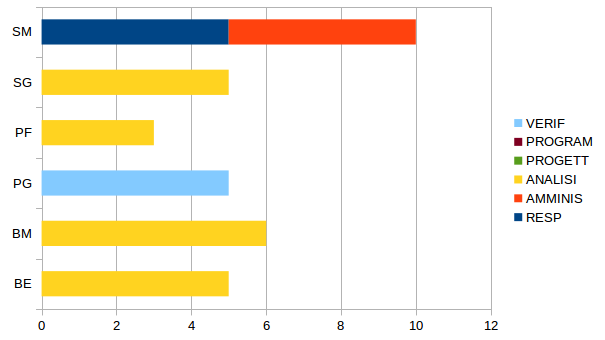
\includegraphics[scale=0.7]{Figures/OreComponenteAnalisiDett.png}
				\caption{Analisi di dettaglio: ore per componente.}\label{fig:4}
			\end{figure}
			\begin{figure}[H]
				\centering
				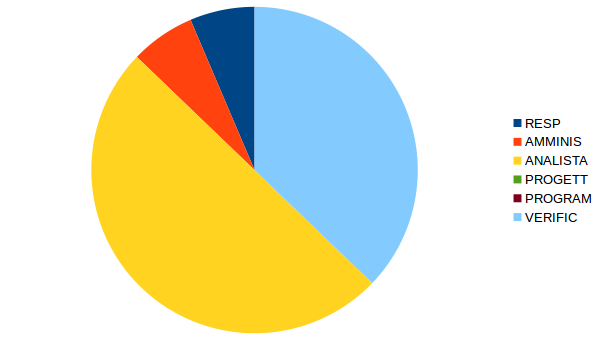
\includegraphics[scale=0.7]{Figures/OreRuoloAnalisiDett.png}
				\caption{Analisi di dettaglio: ore per ruolo.}\label{fig:5}
		\end{figure}
			
			\subsubsection{Prospetto economico}
			\begin{table}[H]
				\center
				\begin{tabular}{|c|c|c|}
					\noalign{\hrule height 1.5pt}
					\textbf{Ruolo} & \textbf{Ore} & \textbf{Costo(\euro)}     \\
					\hline
					Responsabile  & 5 & 150 \\
					\hline
					Amministratore  & 5  & 100 \\
					\hline
					Analista  & 11  & 275\\
					\hline
					Progettista  & 0 & 0\\
					\hline
					Programmatore  & 0 & 0\\
					\hline
					Verificatore  & 12 & 180\\
					\hline
					\textbf{Totale}  & \textbf{33} & \textbf{705}\\
					\noalign{\hrule height 1.5pt}
			\end{tabular}
			\caption{Prospetto economico Analisi di dettaglio.  \label{tab:table_label}}
		\end{table}
		
		
		\subsection{Progettazione architetturale}
			\subsubsection{Prospetto orario}
			\begin{table}[H]
			\center
				\begin{tabular}{cccccccc}
				\noalign{\hrule height 1.5pt}
				\textbf{Nome} & \textbf{Res} & \textbf{Amm} & \textbf{An} & \textbf{Pt} & \textbf{Pr} & \textbf{Ve} & \textbf{Totale} \\ \hline
				Bonato Enrico & - & - & 12 & - & - & 12 & 24 \\ \hline
				Bonolo Marco  & - & 5 & - & 14 & - & - & 19 \\ \hline
				Pace Giulio  & 11 & - & - & 10 & - & - & 21 \\ \hline
				Pezzuto Francesco  & - & - & 9 & 10 & - & - & 19 \\ \hline
				Sanna Giovanni  & - & - & - & 16 & - & - & 16 \\ \hline
				Sovilla Matteo  & - & - & 10 & - & - & 15 & 25 \\ \hline
				\textbf{Ore Totali Ruolo} & \textbf{11} & \textbf{5} & \textbf{31} & \textbf{50} &  \textbf{0}& \textbf{27} & \textbf{124} \\ \hline
				\noalign{\hrule height 1.5pt}
				\end{tabular}
			\caption{Prospetto orario Progettazione architetturale.  \label{tab:table_label}}
			\end{table}
			\begin{figure}[H]
				\centering
				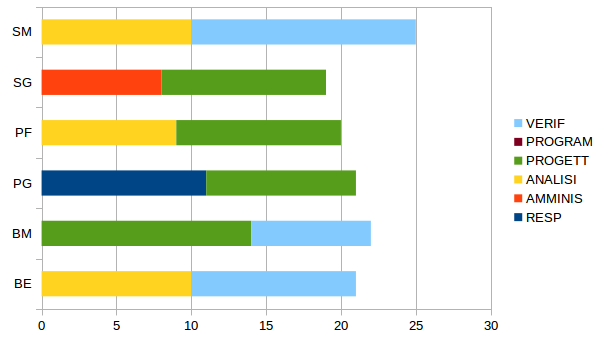
\includegraphics[scale=0.7]{Figures/OreComponenteProgArch.png}
				\caption{Progettazione architetturale: ore per componente.}\label{fig:7}
			\end{figure}
			\begin{figure}[H]
				\centering
				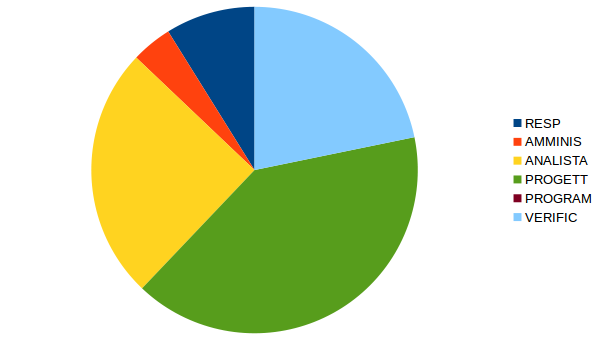
\includegraphics[scale=0.7]{Figures/OreRuoloProgArch.png}
				\caption{Progettazione architetturale: ore per ruolo.}\label{fig:8}
			\end{figure}
			
			\subsubsection{Prospetto economico}
			\begin{table}[H]
				\center
				\begin{tabular}{|c|c|c|}
					\noalign{\hrule height 1.5pt}
					\textbf{Ruolo} & \textbf{Ore} & \textbf{Costo(\euro)}     \\
					\hline
					Responsabile  & 11 & 330 \\
					\hline
					Amministratore  &  5 & 100 \\
					\hline
					Analista  & 31 & 775 \\
					\hline
					Progettista  & 50 & 1100 \\
					\hline
					Programmatore  & 0 & 0 \\
					\hline 
					Verificatore  & 27 & 405 \\
					\hline
					\textbf{Totale}  & \textbf{124} & \textbf{2710}\\
					\noalign{\hrule height 1.5pt}
			\end{tabular}
			\caption{Prospetto economico Progettazione architetturale.  \label{tab:table_label}}
		\end{table}
		
		
		\subsection{Progettazione di dettaglio e Codifica}
			\subsubsection{Prospetto orario}
			\begin{table}[H]
			\center
				\begin{tabular}{cccccccc}
				\noalign{\hrule height 1.5pt}
				\textbf{Nome} & \textbf{Res} & \textbf{Amm} & \textbf{An} & \textbf{Pt} & \textbf{Pr} & \textbf{Ve} & \textbf{Totale} \\ \hline
				Bonato Enrico & - & 5 & - & 22 & 11 & - & 38 \\ \hline
				Bonolo Marco  & 8 & - & - & - & 13 & 25 & 46 \\ \hline
				Pace Giulio  & - & - & - & 17 & 10 & 17 & 44 \\ \hline
				Pezzuto Francesco  & - & 5 & - & 16 & 12 & 14 & 47 \\ \hline
				Sanna Giovanni  & - & - & - & 18 & 12 & 21 & 51 \\ \hline
				Sovilla Matteo  & - & - & 6 & 22 & 17 & - & 45 \\ \hline
				\textbf{Ore Totali Ruolo} & \textbf{8} & \textbf{10} & \textbf{6} & \textbf{95} & \textbf{75} & \textbf{77} & \textbf{271} \\ \hline
				\noalign{\hrule height 1.5pt}
				\end{tabular}
			\caption{Prospetto orario Progettazione di dettaglio e Codifica.  \label{tab:table_label}}
			\end{table}
			\begin{figure}[H]
				\centering
				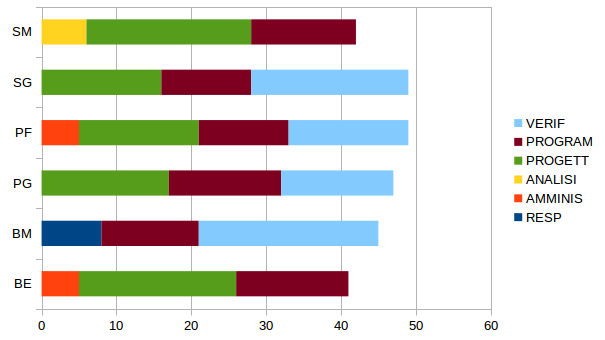
\includegraphics[scale=0.7]{Figures/OreComponenteProgDettCodifica.png}
				\caption{Progettazione di dettaglio e codifica: ore per componente.}\label{fig:10}
			\end{figure}
			\begin{figure}[H]
				\centering
				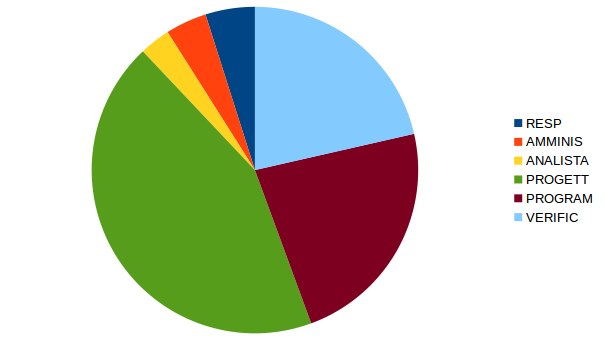
\includegraphics[scale=0.7]{Figures/OreRuoloProgDettCodifica.png}
				\caption{Progettazione di dettaglio e codifica: ore per ruolo.}\label{fig:11}
			\end{figure}
			
			\subsubsection{Prospetto economico}
			\begin{table}[H]
				\center
				\begin{tabular}{|c|c|c|}
					\noalign{\hrule height 1.5pt}
					\textbf{Ruolo} & \textbf{Ore} & \textbf{Costo(\euro)}     \\
					\hline
					Responsabile  & 8 & 240\\
					\hline
					Amministratore  & 10  & 200 \\
					\hline
					Analista  & 6  & 150 \\
					\hline
					Progettista  & 95 & 2090 \\
					\hline
					Programmatore  & 75 & 1125 \\
					\hline
					Verificatore  & 77 & 1155 \\
					\hline
					\textbf{Totale}  & \textbf{271} & \textbf{4960}\\
					\noalign{\hrule height 1.5pt}
			\end{tabular}
			\caption{Prospetto economico Progettazione di dettaglio e Codifica.  \label{tab:table_label}}
		\end{table}
		
		\subsection{Validazione}
			\subsubsection{Prospetto orario}
			\begin{table}[H]
			\center
				\begin{tabular}{cccccccc}
				\noalign{\hrule height 1.5pt}
				\textbf{Nome} & \textbf{Res} & \textbf{Amm} & \textbf{An} & \textbf{Pt} & \textbf{Pr} & \textbf{Ve} & \textbf{Totale} \\ \hline
				Bonato Enrico & - & - & - & 6 & 0 & 14 & 20 \\ \hline
				Bonolo Marco  & - & - & - & 9 & 10 & - & 19 \\ \hline
				Pace Giulio  & - & - & - & - & 7 & 9 & 16 \\ \hline
				Pezzuto Francesco  & 9 & - & - & - & - & 7 & 16 \\ \hline
				Sanna Giovanni  & - & 6 & - & - & 7 & 0 & 13 \\ \hline
				Sovilla Matteo  & - & - & - & - & - & 13 & 13 \\ \hline
				\textbf{Ore Totali Ruolo} & \textbf{9} & \textbf{6} & \textbf{0} & \textbf{15} & \textbf{24} & \textbf{43} & \textbf{97} \\ \hline
				\noalign{\hrule height 1.5pt}
				\end{tabular}
			\caption{Prospetto orario Validazione.  \label{tab:table_label}}
			\end{table}
			\begin{figure}[H]
				\centering
				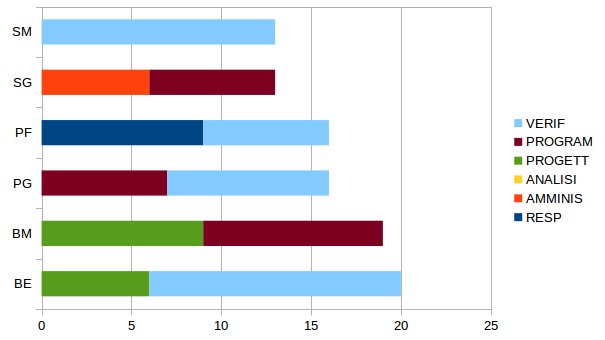
\includegraphics[scale=0.7]{Figures/OreComponenteValidazione.png}
				\caption{Validazione: ore per componente.}\label{fig:13}
			\end{figure}
			\begin{figure}[H]
				\centering
				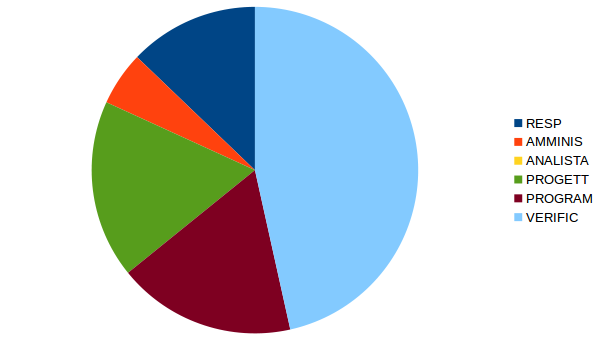
\includegraphics[scale=0.7]{Figures/OreRuoloValidazione.png}
				\caption{Validazione: ore per ruolo.}\label{fig:14}
			\end{figure}
			
			\subsubsection{Prospetto economico}
			\begin{table}[H]
				\center
				\begin{tabular}{|c|c|c|}
					\noalign{\hrule height 1.5pt}
					\textbf{Ruolo} & \textbf{Ore} & \textbf{Costo(\euro)}     \\
					\hline
					Responsabile  & 9 & 270 \\
					\hline
					Amministratore  & 6  & 120 \\
					\hline
					Analista  & 0  & 0 \\
					\hline
					Progettista  & 15 & 330 \\
					\hline
					Programmatore  & 24  & 360\\ 
					\hline
					Verificatore  & 43 & 645 \\
					\hline
					\textbf{Totale}  & \textbf{97} & \textbf{1725}\\
					\noalign{\hrule height 1.5pt}
			\end{tabular}
			\caption{Prospetto economico Validazione.  \label{tab:table_label}}
		\end{table}
		
	\subsection{Riepilogo}
		\subsubsection{Prospetto orario}
		\begin{table}[H]
			\center
				\begin{tabular}{cccccccc}
				\noalign{\hrule height 1.5pt}
				\textbf{Nome} & \textbf{Res} & \textbf{Amm} & \textbf{An} & \textbf{Pt} & \textbf{Pr} & \textbf{Ve} & \textbf{Totale} \\ \hline
				Bonato Enrico & 5 & 10 & 22 & 28 & 11 & 29 & 105 \\ \hline
				Bonolo Marco  & 8 & 5 & 8 & 23 & 23 & 38 & 105 \\ \hline
				Pace Giulio  & 11 & 5 & 8 & 27 & 17 & 37 & 105  \\ \hline
				Pezzuto Francesco  & 9 & 5 & 24 & 26 & 12 & 29 & 105 \\ \hline
				Sanna Giovanni  & 7 & 6 & 14 & 34 & 19 & 25 & 105 \\ \hline
				Sovilla Matteo  & 7 & 5 & 21 & 22 & 17 & 33 & 105 \\ \hline
				\textbf{Ore Totali Ruolo} & \textbf{47} & \textbf{36} & \textbf{97} & \textbf{160} & \textbf{99} & \textbf{191} & \textbf{630} \\ \hline
				\noalign{\hrule height 1.5pt}
				\end{tabular}
			\caption{Riepilogo prospetto orario.  \label{tab:table_label}}
			\end{table}
			\begin{figure}[H]
				\centering
				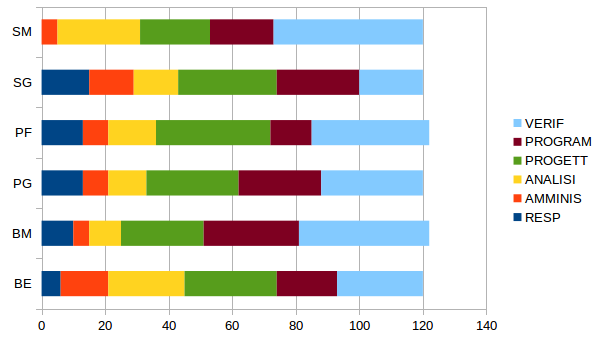
\includegraphics[scale=0.7]{Figures/OreComponenteRiepilogo.png}
				\caption{Riepilogo: ore per componente.}\label{fig:15}
			\end{figure}
			\begin{figure}[H]
				\centering
				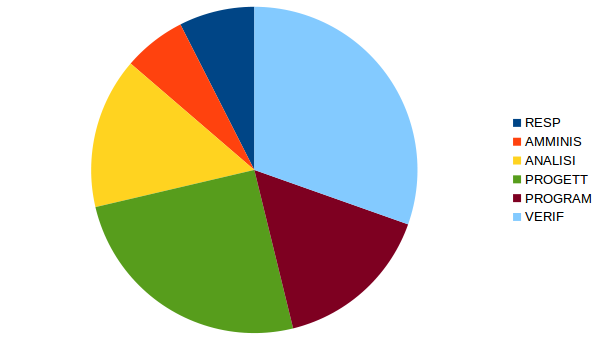
\includegraphics[scale=0.7]{Figures/OreRuoloRiepilogo.png}
				\caption{Riepilogo: ore per ruolo.}\label{fig:5}
			\end{figure}
			
		\subsubsection{Prospetto economico}
			\begin{table}[H]
				\center
				\begin{tabular}{|c|c|c|}
					\noalign{\hrule height 1.5pt}
					\textbf{Ruolo} & \textbf{Ore} & \textbf{Costo(\euro)}     \\
					\hline
					Responsabile  & 47 & 1410 \\ 
					\hline
					Amministratore  & 36  & 720 \\
					\hline
					Analista  & 97  & 2425 \\ 
					\hline
					Progettista  & 160 & 3520\\
					\hline
					Programmatore  & 99  & 1485\\
					\hline
					Verificatore  & 191 & 2865\\
					\hline
					\textbf{Totale}  & \textbf{628} & \textbf{12425}\\
					\noalign{\hrule height 1.5pt}
			\end{tabular}
			\caption{Riepilogo prospetto economico.  \label{tab:table_label}}
		\end{table}
		
\end{document}
